\documentclass[12pt,letterpaper]{exam}
%\usepackage{color}
\usepackage[usenames,dvipsnames,svgnames,table]{xcolor}
\usepackage[margin=0.7in]{geometry}
%\renewcommand{\familydefault}{\sfdefault}
\usepackage{multicol}
\pagestyle{head}
\definecolor{c01}{HTML}{FFBBDD}
\header{MATH 23 }{HW1}{due February 9, 5pm}{}
\runningheadrule
\headrule
\usepackage{diagbox}
\usepackage{graphicx} 
\usepackage{amsmath} 
\usepackage{amssymb} 
\usepackage{hyperref}
\usepackage{enumitem}
\usepackage{MnSymbol}

 \newcommand{\grade}{\textcolor{red}{GRADED}}
 \newcommand{\pts}[1]{\textcolor{red}{[#1]}}
%  \newcommand{\grade}{\textcolor{red}{GRADED}}

%\setlist{nosep} % or \setlist{noitemsep} to leave space around whole list
%\usepackage{sectsty}  % Make section fonts 12 point
%% make a task list:
%\newlist{todolist}{itemize}{2}
%\setlist[todolist]{label=$\square$}
%
%% Adds a vertical column separator.
%\setlength{\columnseprule}{1pt}
%\def\columnseprulecolor{\color{black}}
%
%\sectionfont{\fontsize{13}{15}\selectfont}
%\usepackage{tcolorbox} % Nice boxes

\begin{document}


%%%%%%%%%%%%%%%%%%%%%%%%%%%%%%%%%%%%%%%%%%%%%%%%%%%%
%%%%%%%%%%%%%%%%%%%%%%%%%%%%%%%%%%%%%%%%%%%%%%%%%%%%
%%%%%%%%%%%%%%%%%%%%%%%%%%%%%%%%%%%%%%%%%%%%%%%%%%%%
\section*{Section 1.1}

% --------------------------------------------------------------------------------------------------------------------------------------------
\subsection*{\# 1 \grade \, \pts{2 points}}

 \begin{figure}[h!]
\centering
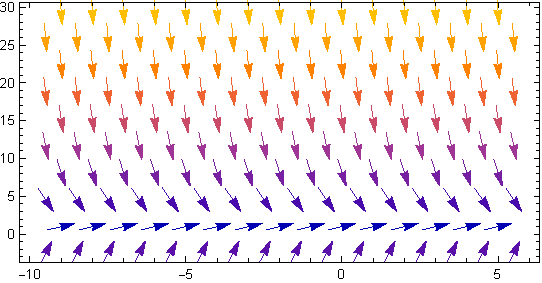
\includegraphics[width=0.5\textwidth]{./1p1_1.pdf}
\end{figure}
\noindent
\pts{Correct drawing of vector field + 1 point}
Regardless of the initial condition, the solution will tend towards $y=3/2$. 
\pts{Long-term behavior + 1 point}

% --------------------------------------------------------------------------------------------------------------------------------------------
\subsection*{\# 3 \grade \, \pts{2 points}}

 \begin{figure}[h!]
\centering
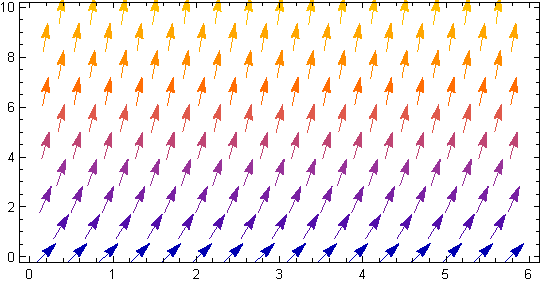
\includegraphics[width=0.5\textwidth]{./1p1_3.pdf}
\end{figure}
\noindent \pts{Correct drawing of vector field + 1 point}
Regardless of the initial condition, the solution tend toward $\infty$.  
\pts{Long-term behavior + 1 point}

% --------------------------------------------------------------------------------------------------------------------------------------------
\subsection*{\# 22 \grade \, \pts{6 points}}

Let $V(t)$ be the volume of the raindrop and $S(t)$ the surface area. The question tells us that 
\begin{equation}
\frac{d}{dt}V(t) = - \gamma S(t)\quad\quad \text{\pts{+1 points}}
\end{equation}
for some number $\gamma$ (the rate per area). If $R$ is the radius, the formula for the volume of a sphere is $V(t) = \frac{4}{3}\pi R^3$ and $S(t) = 4\pi R^2$ \pts{These formulas +2 points} it follows that 
\begin{equation}
S(t) = 4 \pi \left( \frac{3}{4\pi} \right)^{2/3}V^{2/3}  \quad\quad \text{\pts{+1 points}}
\end{equation}
hence 
\begin{equation}
\frac{d}{dt}V(t) = - \mu V^{2/3}  \quad\quad \text{\pts{+2 points}}
\end{equation}
for some constant $\mu$. 


%%%%%%%%%%%%%%%%%%%%%%%%%%%%%%%%%%%%%%%%%%%%%%%%%%%%
%%%%%%%%%%%%%%%%%%%%%%%%%%%%%%%%%%%%%%%%%%%%%%%%%%%%
%%%%%%%%%%%%%%%%%%%%%%%%%%%%%%%%%%%%%%%%%%%%%%%%%%%%
\section*{Section 1.2}

% --------------------------------------------------------------------------------------------------------------------------------------------
\subsection*{\# 7 \grade \, \pts{9 points}}
\begin{enumerate}
\item[(a)] The solution is 
\begin{equation}
p(t) = 900 + ce^{t/2} \quad\quad \text{ \pts{identify solution +2 points}}
\end{equation}
To find $c$ we set $p(0) = 850$: 
\begin{equation}
850 = 900 + c \implies c = -50 \quad\quad \text{\pts{solve for $c$ +1 point} }
\end{equation}
To find the time the population goes extinct, we set $p(t_{\rm ex}) = 0$ and solve for $t_{\rm ex}$: 
\begin{align}
900 -50 e^{t_{\rm ex}/2} =0 &\implies e^{t_{\rm ex}/2}  = \frac{900}{50} =18\\
&\implies t_{\rm ex} = 2 \ln18  \quad\quad \text{\pts{solve for $t_{\rm ex}$ +2 point} }
\end{align}
\item[(b)] The same idea as (a): First find $c$
\begin{equation}
p_0 = 900 + c \implies c = p_0-900
\end{equation}
and find $t_{\rm ex}$
\begin{align}
900 -(p_0-900) e^{t_{\rm ex}/2} =0 &\implies e^{t_{\rm ex}/2}  = \frac{900}{p_0-900}\\
&\implies t_{\rm ex} = 2 \ln\frac{900}{p_0-900} \quad\quad \text{ \pts{repeat (a) with general $p_0$  +2 point} }
\end{align}
\item[(c)]  If $t_{\rm ex} = 1$, 
\begin{align}
t_{\rm ex}  =1= 2 \ln\frac{900}{p_0-900}&\implies  \frac{900}{p_0-900} =e^{1/2}\\
&\implies p_0-900 = \frac{900}{e^{1/2}} \\
&\implies p_0 =   900 + \frac{900}{\ln 2} = 900\left(1+ \frac{1}{e^{1/2}} \right) \quad \text{ \quad \text{\pts{ +2 point}}}
\end{align}

\end{enumerate}


% --------------------------------------------------------------------------------------------------------------------------------------------
\subsection*{\# 12 \grade \, \pts{6 points}}
\begin{enumerate}
\item[(a)] Solving the differential equation for $Q$ yields exponential decay
\begin{equation}\label{eq:10:12a}
Q = Q(0)e^{-rt} \quad \quad \text{\pts{ +1 point}}
\end{equation}
For this problem $Q(0) = 100{\rm mg}$ and at $t=1$ (assuming we measure $t$ in weeks) $Q(t) = 82.04$. Plugging these values in to the solutions yields an equation for $r$: 
\begin{equation}
82.04 = 100 e^{-r} \implies r =  \ln \frac{100}{82.04} \approx 1.97 \quad  \quad \text{\pts{ +2 point}}
\end{equation}
\item[(b)] This is given by Equation \eqref{eq:10:12a} with the values found above:  
\begin{equation}
Q = 100e^{-1.97 t}\quad \quad \text{\pts{ +1 point}}
\end{equation}
\item[(c)] Let $t_{1/2}$ be the time to decay to have the original amount. To find $t_{1/2}$ we solve 
\begin{equation}
Q(t) = \frac{1}{2}Q(0) =Q(0)e^{-rt_{1/2}}   \quad \quad  \text{\pts{ +1 point}}
\end{equation}
which yields 
\begin{equation}
t_{1/2} = - \frac{1}{r} \ln \frac{1}{2} = \frac{1}{r} \ln 2 = \frac{1}{1.97}\ln (2) \quad\quad \text{\pts{ +1 point}}
\end{equation}
\end{enumerate}




%%%%%%%%%%%%%%%%%%%%%%%%%%%%%%%%%%%%%%%%%%%%%%%%%%%%
%%%%%%%%%%%%%%%%%%%%%%%%%%%%%%%%%%%%%%%%%%%%%%%%%%%%
%%%%%%%%%%%%%%%%%%%%%%%%%%%%%%%%%%%%%%%%%%%%%%%%%%%%
\section*{Section 1.3}

% --------------------------------------------------------------------------------------------------------------------------------------------
\subsection*{\# 11 \grade \,\pts{6 points}}
Starting with $y_1$, the derivatives are
\begin{align}
y' &= \frac{1}{2}t^{1/2-1} = \frac{1}{2t^{1/2}} \quad\quad \text{\pts{+1 point}}\\
y'' &= -\frac{1}{2} \frac{1}{2t^{1/2+1}} = -\frac{1}{4t^{3/2}} \quad\quad \text{\pts{+1 point}}
\end{align}
Hence 
\begin{align}
-2t^2y'' + 3ty' - y &= 2\frac{t^2}{4t^{3/2}}  +\frac{3t}{2t^{1/2}} - y\\
&= -\frac{1}{2}t^{1/2} + \frac{3}{2}t^{1/2} - t^{1/2} = t^{1/2} - t^{1/2} \quad\quad \text{\pts{+1 point}}
\end{align}
For $t_2$ we have
\begin{align}
y' &=-t^{-2}  \quad\quad \text{\pts{+1 point}}\\
y'' &= 2 t^{-3} \quad\quad \text{\pts{+1 point}}
\end{align}
hence 
\begin{align}
-4t^{-1} - 3t^{-1}- t^{-1} = 0  \quad\quad \text{\pts{+1 point}}
\end{align}


%%%%%%%%%%%%%%%%%%%%%%%%%%%%%%%%%%%%%%%%%%%%%%%%%%%%
%%%%%%%%%%%%%%%%%%%%%%%%%%%%%%%%%%%%%%%%%%%%%%%%%%%%
%%%%%%%%%%%%%%%%%%%%%%%%%%%%%%%%%%%%%%%%%%%%%%%%%%%%
\section*{Additional Questions}

% --------------------------------------------------------------------------------------------------------------------------------------------




\end{document}


